% ============================================================
% 电路基础实验 —— 实验三 等效电源定理 预习报告
% ============================================================

\documentclass[12pt]{ctexart}

% --- 宏包 ---
\usepackage{graphicx}
\usepackage{amsmath}
\usepackage{float}
\usepackage{booktabs}
\usepackage{siunitx}
\usepackage{caption}
\usepackage{subcaption}
\usepackage{enumitem}

\sisetup{per-mode=symbol}

\graphicspath{{./figures/}{../requirements/extracted_images/word/media/}{./}}

\usepackage[left=2.5cm, right=2.5cm, top=2.5cm, bottom=2.5cm]{geometry}

\setlength{\jot}{6pt}
\linespread{1.5}
\setlist{nosep}

\begin{document}

% ==================== 封面 ====================
\thispagestyle{empty}

\begin{center}
    \LARGE\textbf{第3次实验\ 验证等效电源定理预习报告}

    \vspace{1cm}
    \normalsize
    组名：第7组\quad 姓名：郭浩然\quad 学号：2024303980
\end{center}

\vspace{1cm}

% ==================== 正文 ====================

% (10) 实验目的
\section{实验目的}

\begin{enumerate}[label=\arabic*.]
    \item 学习并验证戴维南定理，理解线性有源单口网络对外等效的意义。
    \item 掌握等效电源内阻的多种测量方法，包括直接测量法、开路短路法、二次测量法和半偏法。
    \item 学习可调电阻作为负载的使用方法，通过改变负载比较原电路与等效电路的端口伏安特性。
\end{enumerate}

% (80) 实验原理
\section{实验原理}

\subsection{戴维南定理}

戴维南定理指出，任意线性有源单口网络，从外部端口看，都可以等效为一个理想电压源与一个电阻串联的形式。该理想电压源的电压等于原网络端口的开路电压，串联电阻等于原网络中所有独立源置零后从端口看进去的等效电阻。其等效形式可表示为
\begin{equation}
    U = U_{oc} - I R_{\mathrm{th}},
\end{equation}
其中，\(U_{oc}\) 为端口开路电压，\(R_{\mathrm{th}}\) 为戴维南等效内阻，\(U\) 和 \(I\) 分别为外接负载时端口电压和端口电流。

求取戴维南等效电阻时，需要将原网络中的独立源置零：理想电压源用短路代替，理想电流源用开路代替。若网络中含受控源，则受控源不能置零，应保留其控制关系。

\subsection{等效内阻测量方法}

本实验涉及多种等效内阻测量方法，各方法原理如下。

\subsubsection{直接测量法}

将有源网络中的独立电源置零后，从端口处用万用表欧姆档直接测量等效电阻。该方法操作简单，但要求电路断电，且测量结果会受到仪表内部测量方式和电路连接状态的影响。

\subsubsection{开路短路法}

先测量端口开路时的电压 \(U_{oc}\)，再测量端口短路时的短路电流 \(I_{sc}\)。由戴维南等效电路可得
\begin{equation}
    R_{\mathrm{th}}=\frac{U_{oc}}{I_{sc}}.
\end{equation}
该方法物理意义明确，但短路测量时电流可能较大，实验中应注意量程和电路安全。

\subsubsection{二次测量法}

先测量端口开路电压 \(U_{oc}\)，再接入已知负载 \(R_L\)，测量负载端电压 \(U_L\)。根据分压关系有
\begin{equation}
    U_L = U_{oc}\frac{R_L}{R_{\mathrm{th}}+R_L},
\end{equation}
因此
\begin{equation}
    R_{\mathrm{th}}=R_L\left(\frac{U_{oc}}{U_L}-1\right).
\end{equation}
该方法不需要短接端口，适合对短路电流较敏感的电路。

\subsubsection{半偏法}

半偏法通过调节负载电阻，使负载端电压或电流达到某一参考值的一半。对于戴维南等效电路，当负载电阻 \(R_L\) 等于等效内阻 \(R_{\mathrm{th}}\) 时，负载电压为开路电压的一半：
\begin{equation}
    U_L=\frac{U_{oc}}{2}\quad\Longrightarrow\quad R_L=R_{\mathrm{th}}.
\end{equation}
因此可通过调节可变负载并观察负载电压变化，估算等效内阻。

\subsection{实验电路与 Multisim 仿真}

实验三的 Multisim 仿真电路如图~\ref{fig:thevenin-multisim} 所示。实验时先对原线性有源网络进行开路电压、短路电流和负载端口伏安特性测量，再根据测得的 \(U_{oc}\) 与 \(R_{\mathrm{th}}\) 搭建戴维南等效电路，并比较原电路和等效电路在不同负载下的端口电压与电流。

\begin{figure}[H]
    \centering
    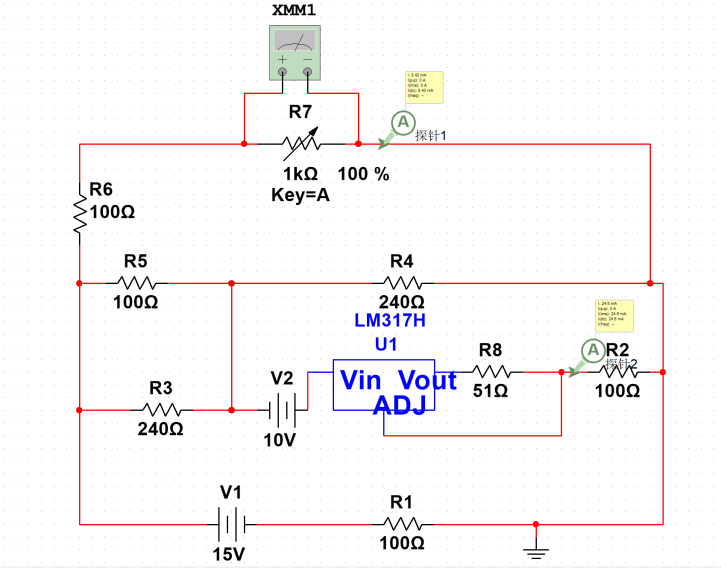
\includegraphics[width=0.78\textwidth]{image6.png}
    \caption{实验三 Multisim 仿真电路}
    \label{fig:thevenin-multisim}
\end{figure}

\subsection{Multisim 仿真结果}

根据参考仿真结果，原网络端口开路电压和短路电流分别为
\begin{align}
    U_{oc} &= 9.909\,\mathrm{V}, \\
    I_{sc} &= 55.76\,\mathrm{mA}.
\end{align}
由开路短路法可得等效内阻
\begin{equation}
    R_{\mathrm{th}}=\frac{U_{oc}}{I_{sc}}
    =\frac{9.909\,\mathrm{V}}{55.76\,\mathrm{mA}}
    \approx 177.71\,\Omega.
\end{equation}

改变负载电阻时，原电路与戴维南等效电路的端口测量结果如表~\ref{tab:simulation-result} 所示。两组数据接近，说明在外部端口看来，戴维南等效电路能够较好地替代原线性有源网络。

\begin{table}[H]
    \centering
    \caption{原电路与戴维南等效电路仿真结果对比}
    \label{tab:simulation-result}
    \begin{tabular}{ccccc}
        \toprule
        负载电阻/\(\Omega\) & 原电路 \(U\)/V & 原电路 \(I\)/mA & 等效电路 \(U\)/V & 等效电路 \(I\)/mA \\
        \midrule
        100 & 3.620 & 36.30 & 3.545 & 35.52 \\
        510 & 7.352 & 14.42 & 7.325 & 14.42 \\
        1000 & 8.432 & 8.52 & 8.366 & 8.32 \\
        \bottomrule
    \end{tabular}
\end{table}

从表中可见，负载变化时，原电路和等效电路的端口电压、电流均随负载呈一致变化趋势，二者偏差较小。实验中可进一步通过绘制 \(U-I\) 曲线比较两者的斜率和截距，以验证等效电源定理。

% (10) 实验器件
\section{实验器件}

\begin{itemize}
    \item 面包板 \(\times 1\)
    \item 可编程直流电源 \(\times 1\)
    \item 数字万用表 \(\times 1\)
    \item 电阻：\(51\,\Omega\times 1\)、\(100\,\Omega\times 4\)、\(240\,\Omega\times 2\)
    \item 可调电阻或可变负载 \(\times 1\)
    \item 导线若干
\end{itemize}

\end{document}
